\documentclass{book}
\usepackage[a4paper,top=2.5cm,bottom=2.5cm,left=2.5cm,right=2.5cm]{geometry}
\usepackage{makeidx}
\usepackage{natbib}
\usepackage{graphicx}
\usepackage{multicol}
\usepackage{float}
\usepackage{listings}
\usepackage{color}
\usepackage{ifthen}
\usepackage[table]{xcolor}
\usepackage{textcomp}
\usepackage{alltt}
\usepackage{ifpdf}
\ifpdf
\usepackage[pdftex,
            pagebackref=true,
            colorlinks=true,
            linkcolor=blue,
            unicode
           ]{hyperref}
\else
\usepackage[ps2pdf,
            pagebackref=true,
            colorlinks=true,
            linkcolor=blue,
            unicode
           ]{hyperref}
\usepackage{pspicture}
\fi
\usepackage[utf8]{inputenc}
\usepackage{mathptmx}
\usepackage[scaled=.90]{helvet}
\usepackage{courier}
\usepackage{sectsty}
\usepackage{amssymb}
\usepackage[titles]{tocloft}
\usepackage{doxygen}
\lstset{language=C++,inputencoding=utf8,basicstyle=\footnotesize,breaklines=true,breakatwhitespace=true,tabsize=4,numbers=left }
\makeindex
\setcounter{tocdepth}{3}
\renewcommand{\footrulewidth}{0.4pt}
\renewcommand{\familydefault}{\sfdefault}
\hfuzz=15pt
\setlength{\emergencystretch}{15pt}
\hbadness=750
\tolerance=750
\begin{document}
\hypersetup{pageanchor=false,citecolor=blue}
\begin{titlepage}
\vspace*{7cm}
\begin{center}
{\Large Apriori All }\\
\vspace*{1cm}
{\large Generated by Doxygen 1.8.2}\\
\vspace*{0.5cm}
{\small Tue Nov 27 2012 17:43:34}\\
\end{center}
\end{titlepage}
\clearemptydoublepage
\pagenumbering{roman}
\tableofcontents
\clearemptydoublepage
\pagenumbering{arabic}
\hypersetup{pageanchor=true,citecolor=blue}
\chapter{Namespace Index}
\section{Packages}
Here are the packages with brief descriptions (if available)\-:\begin{DoxyCompactList}
\item\contentsline{section}{\hyperlink{namespace_apriori_all_lib}{Apriori\-All\-Lib} }{\pageref{namespace_apriori_all_lib}}{}
\end{DoxyCompactList}

\chapter{Hierarchical Index}
\section{Class Hierarchy}
This inheritance list is sorted roughly, but not completely, alphabetically\-:\begin{DoxyCompactList}
\item \contentsline{section}{Apriori\-All\-Lib.\-Apriori}{\pageref{class_apriori_all_lib_1_1_apriori}}{}
\item \contentsline{section}{Apriori\-All\-Lib.\-Apriori\-All\-Algorithm}{\pageref{class_apriori_all_lib_1_1_apriori_all_algorithm}}{}
\item \contentsline{section}{Apriori\-All\-Lib.\-Customer}{\pageref{class_apriori_all_lib_1_1_customer}}{}
\item \contentsline{section}{Apriori\-All\-Lib.\-Customer\-List}{\pageref{class_apriori_all_lib_1_1_customer_list}}{}
\item I\-Comparable\begin{DoxyCompactList}
\item \contentsline{section}{Apriori\-All\-Lib.\-Item}{\pageref{class_apriori_all_lib_1_1_item}}{}
\item \contentsline{section}{Apriori\-All\-Lib.\-Litemset}{\pageref{class_apriori_all_lib_1_1_litemset}}{}
\end{DoxyCompactList}
\item \contentsline{section}{Apriori\-All\-Lib.\-Transaction}{\pageref{class_apriori_all_lib_1_1_transaction}}{}
\item \contentsline{section}{Apriori\-All\-Lib.\-Xml\-Reader}{\pageref{class_apriori_all_lib_1_1_xml_reader}}{}
\end{DoxyCompactList}

\chapter{Class Index}
\section{Class List}
Here are the classes, structs, unions and interfaces with brief descriptions\-:\begin{DoxyCompactList}
\item\contentsline{section}{\hyperlink{class_apriori_all_lib_1_1_apriori}{Apriori\-All\-Lib.\-Apriori} \\*This class is used for calculating litemsets from a set of customers' transactions }{\pageref{class_apriori_all_lib_1_1_apriori}}{}
\item\contentsline{section}{\hyperlink{class_apriori_all_lib_1_1_apriori_all_algorithm}{Apriori\-All\-Lib.\-Apriori\-All\-Algorithm} \\*\hyperlink{class_apriori_all_lib_1_1_apriori}{Apriori} All Algorithm \-:P }{\pageref{class_apriori_all_lib_1_1_apriori_all_algorithm}}{}
\item\contentsline{section}{\hyperlink{class_apriori_all_lib_1_1_customer}{Apriori\-All\-Lib.\-Customer} \\*Class which represents a customer from database having a list of transactions }{\pageref{class_apriori_all_lib_1_1_customer}}{}
\item\contentsline{section}{\hyperlink{class_apriori_all_lib_1_1_customer_list}{Apriori\-All\-Lib.\-Customer\-List} \\*Class that represents a total set of customers }{\pageref{class_apriori_all_lib_1_1_customer_list}}{}
\item\contentsline{section}{\hyperlink{class_apriori_all_lib_1_1_item}{Apriori\-All\-Lib.\-Item} \\*Single item of a transaction. }{\pageref{class_apriori_all_lib_1_1_item}}{}
\item\contentsline{section}{\hyperlink{class_apriori_all_lib_1_1_litemset}{Apriori\-All\-Lib.\-Litemset} \\*Class that represents a litemset (1-\/itemset) }{\pageref{class_apriori_all_lib_1_1_litemset}}{}
\item\contentsline{section}{\hyperlink{class_apriori_all_lib_1_1_transaction}{Apriori\-All\-Lib.\-Transaction} \\*Single client's transaction having a list of items }{\pageref{class_apriori_all_lib_1_1_transaction}}{}
\item\contentsline{section}{\hyperlink{class_apriori_all_lib_1_1_xml_reader}{Apriori\-All\-Lib.\-Xml\-Reader} \\*Class that reads data from xml client database and transforms them into classes }{\pageref{class_apriori_all_lib_1_1_xml_reader}}{}
\end{DoxyCompactList}

\chapter{Namespace Documentation}
\hypertarget{namespace_apriori_all_lib}{\section{Package Apriori\-All\-Lib}
\label{namespace_apriori_all_lib}\index{Apriori\-All\-Lib@{Apriori\-All\-Lib}}
}
\subsection*{Classes}
\begin{DoxyCompactItemize}
\item 
class \hyperlink{class_apriori_all_lib_1_1_apriori}{Apriori}
\begin{DoxyCompactList}\small\item\em This class is used for calculating litemsets from a set of customers' transactions \end{DoxyCompactList}\item 
class \hyperlink{class_apriori_all_lib_1_1_apriori_all_algorithm}{Apriori\-All\-Algorithm}
\begin{DoxyCompactList}\small\item\em \hyperlink{class_apriori_all_lib_1_1_apriori}{Apriori} All Algorithm \-:P \end{DoxyCompactList}\item 
class \hyperlink{class_apriori_all_lib_1_1_customer}{Customer}
\begin{DoxyCompactList}\small\item\em Class which represents a customer from database having a list of transactions \end{DoxyCompactList}\item 
class \hyperlink{class_apriori_all_lib_1_1_customer_list}{Customer\-List}
\begin{DoxyCompactList}\small\item\em Class that represents a total set of customers \end{DoxyCompactList}\item 
class \hyperlink{class_apriori_all_lib_1_1_item}{Item}
\begin{DoxyCompactList}\small\item\em Single item of a transaction. \end{DoxyCompactList}\item 
class \hyperlink{class_apriori_all_lib_1_1_litemset}{Litemset}
\begin{DoxyCompactList}\small\item\em Class that represents a litemset (1-\/itemset) \end{DoxyCompactList}\item 
class \hyperlink{class_apriori_all_lib_1_1_transaction}{Transaction}
\begin{DoxyCompactList}\small\item\em Single client's transaction having a list of items \end{DoxyCompactList}\item 
class \hyperlink{class_apriori_all_lib_1_1_xml_reader}{Xml\-Reader}
\begin{DoxyCompactList}\small\item\em Class that reads data from xml client database and transforms them into classes \end{DoxyCompactList}\end{DoxyCompactItemize}

\chapter{Class Documentation}
\hypertarget{class_apriori_all_lib_1_1_apriori}{\section{Apriori\-All\-Lib.\-Apriori Class Reference}
\label{class_apriori_all_lib_1_1_apriori}\index{Apriori\-All\-Lib.\-Apriori@{Apriori\-All\-Lib.\-Apriori}}
}


This class is used for calculating litemsets from a set of customers' transactions  




Collaboration diagram for Apriori\-All\-Lib.\-Apriori\-:
\nopagebreak
\begin{figure}[H]
\begin{center}
\leavevmode
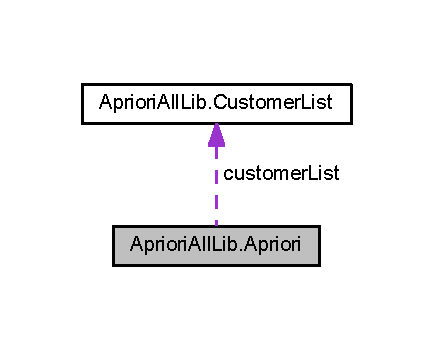
\includegraphics[width=208pt]{class_apriori_all_lib_1_1_apriori__coll__graph}
\end{center}
\end{figure}
\subsection*{Public Member Functions}
\begin{DoxyCompactItemize}
\item 
\hyperlink{class_apriori_all_lib_1_1_apriori_a07c440217ce84e547c31c71ba9a2742e}{Apriori} (\hyperlink{class_apriori_all_lib_1_1_customer_list}{Customer\-List} \hyperlink{class_apriori_all_lib_1_1_apriori_abbca8be3761136e76782ce10ebd61638}{customer\-List})
\begin{DoxyCompactList}\small\item\em Constructor \end{DoxyCompactList}\item 
List$<$ \hyperlink{class_apriori_all_lib_1_1_litemset}{Litemset} $>$ \hyperlink{class_apriori_all_lib_1_1_apriori_a64e63d73cfc770ef8532127198b314dd}{Find\-One\-Litemsets} (double minimal\-Support)
\begin{DoxyCompactList}\small\item\em Finds all litemsets that have the minimal support \end{DoxyCompactList}\end{DoxyCompactItemize}
\subsection*{Private Member Functions}
\begin{DoxyCompactItemize}
\item 
List$<$ \hyperlink{class_apriori_all_lib_1_1_litemset}{Litemset} $>$ \hyperlink{class_apriori_all_lib_1_1_apriori_a79d720678f873cfb665fe6cbf4bf32ae}{generate\-Candidates} (List$<$ \hyperlink{class_apriori_all_lib_1_1_item}{Item} $>$ items)
\begin{DoxyCompactList}\small\item\em Produces all subsets of a given list of items in a transaction \end{DoxyCompactList}\end{DoxyCompactItemize}
\subsection*{Private Attributes}
\begin{DoxyCompactItemize}
\item 
\hyperlink{class_apriori_all_lib_1_1_customer_list}{Customer\-List} \hyperlink{class_apriori_all_lib_1_1_apriori_abbca8be3761136e76782ce10ebd61638}{customer\-List}
\end{DoxyCompactItemize}


\subsection{Detailed Description}
This class is used for calculating litemsets from a set of customers' transactions 



\subsection{Constructor \& Destructor Documentation}
\hypertarget{class_apriori_all_lib_1_1_apriori_a07c440217ce84e547c31c71ba9a2742e}{\index{Apriori\-All\-Lib\-::\-Apriori@{Apriori\-All\-Lib\-::\-Apriori}!Apriori@{Apriori}}
\index{Apriori@{Apriori}!AprioriAllLib::Apriori@{Apriori\-All\-Lib\-::\-Apriori}}
\subsubsection[{Apriori}]{\setlength{\rightskip}{0pt plus 5cm}Apriori\-All\-Lib.\-Apriori.\-Apriori (
\begin{DoxyParamCaption}
\item[{{\bf Customer\-List}}]{customer\-List}
\end{DoxyParamCaption}
)}}\label{class_apriori_all_lib_1_1_apriori_a07c440217ce84e547c31c71ba9a2742e}


Constructor 


\begin{DoxyParams}{Parameters}
{\em customer\-List} & \hyperlink{class_apriori_all_lib_1_1_customer_list}{Customer\-List} object containing a list of Customers from a database\\
\hline
\end{DoxyParams}

\begin{DoxyCode}
        \{
            this.\hyperlink{class_apriori_all_lib_1_1_apriori_abbca8be3761136e76782ce10ebd61638}{customerList} = \hyperlink{class_apriori_all_lib_1_1_apriori_abbca8be3761136e76782ce10ebd61638}{customerList};
        \}
\end{DoxyCode}


\subsection{Member Function Documentation}
\hypertarget{class_apriori_all_lib_1_1_apriori_a64e63d73cfc770ef8532127198b314dd}{\index{Apriori\-All\-Lib\-::\-Apriori@{Apriori\-All\-Lib\-::\-Apriori}!Find\-One\-Litemsets@{Find\-One\-Litemsets}}
\index{Find\-One\-Litemsets@{Find\-One\-Litemsets}!AprioriAllLib::Apriori@{Apriori\-All\-Lib\-::\-Apriori}}
\subsubsection[{Find\-One\-Litemsets}]{\setlength{\rightskip}{0pt plus 5cm}List$<${\bf Litemset}$>$ Apriori\-All\-Lib.\-Apriori.\-Find\-One\-Litemsets (
\begin{DoxyParamCaption}
\item[{double}]{minimal\-Support}
\end{DoxyParamCaption}
)}}\label{class_apriori_all_lib_1_1_apriori_a64e63d73cfc770ef8532127198b314dd}


Finds all litemsets that have the minimal support 


\begin{DoxyParams}{Parameters}
{\em minimal\-Support} & Minimal support\\
\hline
\end{DoxyParams}
\begin{DoxyReturn}{Returns}
A list of Litemsets with support $>$= minimal\-Support
\end{DoxyReturn}

\begin{DoxyCode}
        \{
            \textcolor{keywordflow}{if} (minimalSupport > 1 || minimalSupport < 0)
                \textcolor{keywordflow}{return} null; 
            
            minimalSupport *= \hyperlink{class_apriori_all_lib_1_1_apriori_abbca8be3761136e76782ce10ebd61638}{customerList}.\hyperlink{class_apriori_all_lib_1_1_customer_list_a4fd2a16a984844e61ffc60b327e6534a}{Customers}.Count
      ;
            List<Litemset> litemsets = \textcolor{keyword}{new} List<Litemset>();

            \textcolor{keywordflow}{foreach} (Customer c \textcolor{keywordflow}{in} \hyperlink{class_apriori_all_lib_1_1_apriori_abbca8be3761136e76782ce10ebd61638}{customerList}.\hyperlink{class_apriori_all_lib_1_1_customer_list_a4fd2a16a984844e61ffc60b327e6534a}{Customers})
            \{
                \textcolor{keywordflow}{foreach} (Transaction t \textcolor{keywordflow}{in} c.Transactions)
                \{
                    \textcolor{comment}{//generate subsets (candidates for litemsets)}
                    List<Litemset> candidateLitemsets = \hyperlink{class_apriori_all_lib_1_1_apriori_a79d720678f873cfb665fe6cbf4bf32ae}{generateCandidates}
      (t.Items);

                    \textcolor{comment}{//check if they already exist in litemsets list; if not,
       add a litemset to litemsets}
                    \textcolor{keywordflow}{foreach} (Litemset lset \textcolor{keywordflow}{in} candidateLitemsets)
                    \{
                        IEnumerable<Litemset> l = litemsets.Where(litemset => (
      litemset.Items.Count == lset.Items.Count) &&
                            litemset.Items.All(item => lset.Items.Exists(
      lsetItem => lsetItem.CompareTo(item) == 0)));

                        \textcolor{keywordtype}{int} custID = \hyperlink{class_apriori_all_lib_1_1_apriori_abbca8be3761136e76782ce10ebd61638}{customerList}.\hyperlink{class_apriori_all_lib_1_1_customer_list_a4fd2a16a984844e61ffc60b327e6534a}{Customers}
      .IndexOf(c);
                        \textcolor{keywordflow}{if} (l.Count() == 0 && !lset.IDs.Contains(custID))
                        \{
                            litemsets.Add(lset);
                            lset.Support++;
                            lset.IDs.Add(custID);
                        \}
                        \textcolor{keywordflow}{else}
                        \{
                            Litemset litset = l.FirstOrDefault();
                            \textcolor{keywordflow}{if} (!litset.IDs.Contains(custID))
                            \{
                                litset.Support++;
                                litset.IDs.Add(custID);
                            \}
                        \}     
                    \}
                \}
            \}
            \textcolor{comment}{// rewrite the litemsets with support >= minimum to a new list}
            List<Litemset> properLitemsets = \textcolor{keyword}{new} List<Litemset>();
            \textcolor{keywordflow}{foreach} (Litemset litemset \textcolor{keywordflow}{in} litemsets)
                \textcolor{keywordflow}{if} (litemset.Support >= minimalSupport)
                    properLitemsets.Add(litemset);

            properLitemsets.Sort();

            \textcolor{keywordflow}{return} properLitemsets;
        \}
\end{DoxyCode}


Here is the call graph for this function\-:
\nopagebreak
\begin{figure}[H]
\begin{center}
\leavevmode
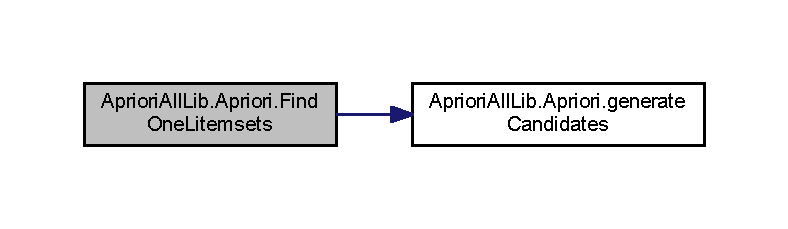
\includegraphics[width=350pt]{class_apriori_all_lib_1_1_apriori_a64e63d73cfc770ef8532127198b314dd_cgraph}
\end{center}
\end{figure}




Here is the caller graph for this function\-:\nopagebreak
\begin{figure}[H]
\begin{center}
\leavevmode
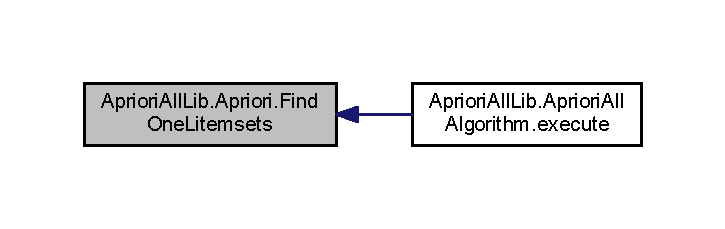
\includegraphics[width=348pt]{class_apriori_all_lib_1_1_apriori_a64e63d73cfc770ef8532127198b314dd_icgraph}
\end{center}
\end{figure}


\hypertarget{class_apriori_all_lib_1_1_apriori_a79d720678f873cfb665fe6cbf4bf32ae}{\index{Apriori\-All\-Lib\-::\-Apriori@{Apriori\-All\-Lib\-::\-Apriori}!generate\-Candidates@{generate\-Candidates}}
\index{generate\-Candidates@{generate\-Candidates}!AprioriAllLib::Apriori@{Apriori\-All\-Lib\-::\-Apriori}}
\subsubsection[{generate\-Candidates}]{\setlength{\rightskip}{0pt plus 5cm}List$<${\bf Litemset}$>$ Apriori\-All\-Lib.\-Apriori.\-generate\-Candidates (
\begin{DoxyParamCaption}
\item[{List$<$ {\bf Item} $>$}]{items}
\end{DoxyParamCaption}
)\hspace{0.3cm}{\ttfamily [private]}}}\label{class_apriori_all_lib_1_1_apriori_a79d720678f873cfb665fe6cbf4bf32ae}


Produces all subsets of a given list of items in a transaction 


\begin{DoxyParams}{Parameters}
{\em items} & List of items contained in one transaction\\
\hline
\end{DoxyParams}
\begin{DoxyReturn}{Returns}
List of Litemsets
\end{DoxyReturn}

\begin{DoxyCode}
        \{
            \textcolor{keywordtype}{int} count = items.Count;
            \textcolor{keywordtype}{int} i = 0;
            List<List<Item>> candLitemsets = \textcolor{keyword}{new} List<List<Item>>();

            \textcolor{comment}{// add a frequent sequence containing all the elements in this
       transaction}
            candLitemsets.Add(\textcolor{keyword}{new} List<Item>(items));
            count--;
            \textcolor{keywordflow}{while} (count != 0)
            \{
                List<Item> temp;
                \textcolor{keywordflow}{foreach} (Item item \textcolor{keywordflow}{in} candLitemsets[i])
                \{
                    temp = \textcolor{keyword}{new} List<Item>(candLitemsets[i]);
                    temp.Remove(item);
                    \textcolor{comment}{// check if there's already such subsequence in the list,
       add}
                    \textcolor{comment}{// if it doesn't exist}
                    \textcolor{keywordflow}{if} (!candLitemsets.Exists(list => list.Count == count &&
                        temp.All(tempItem => list.Exists(listItem => listItem.
      CompareTo(tempItem) == 0))))
                        candLitemsets.Add(temp);
                \}
                \textcolor{keywordflow}{if} (candLitemsets[i + 1].Count == candLitemsets[i].Count - 1)
                    count--;
                i++;
            \}
            List<Litemset> l = \textcolor{keyword}{new} List<Litemset>();
            \textcolor{keywordflow}{foreach} (List<Item> j \textcolor{keywordflow}{in} candLitemsets)
                l.Add(\textcolor{keyword}{new} Litemset(j));
            \textcolor{keywordflow}{return} l;
        \}
\end{DoxyCode}


Here is the caller graph for this function\-:
\nopagebreak
\begin{figure}[H]
\begin{center}
\leavevmode
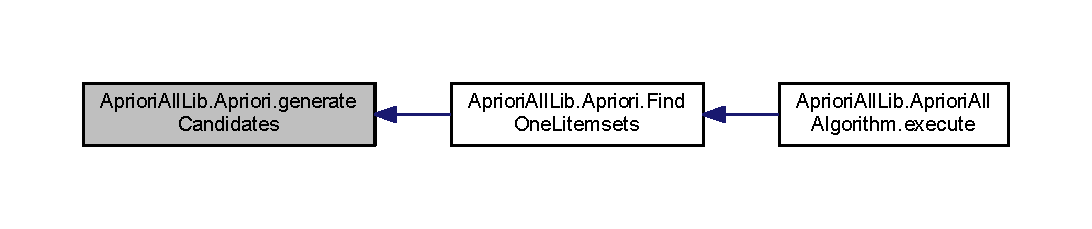
\includegraphics[width=350pt]{class_apriori_all_lib_1_1_apriori_a79d720678f873cfb665fe6cbf4bf32ae_icgraph}
\end{center}
\end{figure}




\subsection{Member Data Documentation}
\hypertarget{class_apriori_all_lib_1_1_apriori_abbca8be3761136e76782ce10ebd61638}{\index{Apriori\-All\-Lib\-::\-Apriori@{Apriori\-All\-Lib\-::\-Apriori}!customer\-List@{customer\-List}}
\index{customer\-List@{customer\-List}!AprioriAllLib::Apriori@{Apriori\-All\-Lib\-::\-Apriori}}
\subsubsection[{customer\-List}]{\setlength{\rightskip}{0pt plus 5cm}{\bf Customer\-List} Apriori\-All\-Lib.\-Apriori.\-customer\-List\hspace{0.3cm}{\ttfamily [private]}}}\label{class_apriori_all_lib_1_1_apriori_abbca8be3761136e76782ce10ebd61638}


The documentation for this class was generated from the following file\-:\begin{DoxyCompactItemize}
\item 
D\-:/\-Projects/\-Csharp/\-Mi\-N\-I\-\_\-\-Apriori\-All/\-Apriori\-All\-Lib/\hyperlink{_apriori_8cs}{Apriori.\-cs}\end{DoxyCompactItemize}

\hypertarget{class_apriori_all_lib_1_1_apriori_all_algorithm}{\section{Apriori\-All\-Lib.\-Apriori\-All\-Algorithm Class Reference}
\label{class_apriori_all_lib_1_1_apriori_all_algorithm}\index{Apriori\-All\-Lib.\-Apriori\-All\-Algorithm@{Apriori\-All\-Lib.\-Apriori\-All\-Algorithm}}
}


\hyperlink{class_apriori_all_lib_1_1_apriori}{Apriori} All Algorithm \-:P  


\subsection*{Static Public Member Functions}
\begin{DoxyCompactItemize}
\item 
static List$<$ \hyperlink{class_apriori_all_lib_1_1_customer}{Customer} $>$ \hyperlink{class_apriori_all_lib_1_1_apriori_all_algorithm_ae4f86f8c88052d29cbfc629f2f61c302}{execute} (\hyperlink{class_apriori_all_lib_1_1_customer_list}{Customer\-List} customer\-List, double threshold)
\begin{DoxyCompactList}\small\item\em Executes \hyperlink{class_apriori_all_lib_1_1_apriori}{Apriori} All algorithm on a given input and minimum suport threshold. \end{DoxyCompactList}\end{DoxyCompactItemize}


\subsection{Detailed Description}
\hyperlink{class_apriori_all_lib_1_1_apriori}{Apriori} All Algorithm \-:P 



\subsection{Member Function Documentation}
\hypertarget{class_apriori_all_lib_1_1_apriori_all_algorithm_ae4f86f8c88052d29cbfc629f2f61c302}{\index{Apriori\-All\-Lib\-::\-Apriori\-All\-Algorithm@{Apriori\-All\-Lib\-::\-Apriori\-All\-Algorithm}!execute@{execute}}
\index{execute@{execute}!AprioriAllLib::AprioriAllAlgorithm@{Apriori\-All\-Lib\-::\-Apriori\-All\-Algorithm}}
\subsubsection[{execute}]{\setlength{\rightskip}{0pt plus 5cm}static List$<${\bf Customer}$>$ Apriori\-All\-Lib.\-Apriori\-All\-Algorithm.\-execute (
\begin{DoxyParamCaption}
\item[{{\bf Customer\-List}}]{customer\-List, }
\item[{double}]{threshold}
\end{DoxyParamCaption}
)\hspace{0.3cm}{\ttfamily [static]}}}\label{class_apriori_all_lib_1_1_apriori_all_algorithm_ae4f86f8c88052d29cbfc629f2f61c302}


Executes \hyperlink{class_apriori_all_lib_1_1_apriori}{Apriori} All algorithm on a given input and minimum suport threshold. 


\begin{DoxyParams}{Parameters}
{\em list} & list of customers, who have transactions that have items\\
\hline
{\em threshold} & from 0 to 1\\
\hline
\end{DoxyParams}
\begin{DoxyReturn}{Returns}

\end{DoxyReturn}


The documentation for this class was generated from the following file\-:\begin{DoxyCompactItemize}
\item 
C\-:/\-Users/\-Karolina/\-Desktop/\-Apriori -\/ Copy/\-Apriori\-All\-Lib/Apriori\-All\-Algorithm.\-cs\end{DoxyCompactItemize}

\hypertarget{class_apriori_all_lib_1_1_customer}{\section{Apriori\-All\-Lib.\-Customer Class Reference}
\label{class_apriori_all_lib_1_1_customer}\index{Apriori\-All\-Lib.\-Customer@{Apriori\-All\-Lib.\-Customer}}
}


Class which represents a customer from database having a list of transactions  


\subsection*{Public Member Functions}
\begin{DoxyCompactItemize}
\item 
\hyperlink{class_apriori_all_lib_1_1_customer_af02616d948989c7ff6161efc2488ecab}{Customer} ()
\begin{DoxyCompactList}\small\item\em Constructor \end{DoxyCompactList}\item 
\hyperlink{class_apriori_all_lib_1_1_customer_a168c8ef2fa0b53671ea51fa21d788f7e}{Customer} (params \hyperlink{class_apriori_all_lib_1_1_transaction}{Transaction}\mbox{[}$\,$\mbox{]} transactions)
\begin{DoxyCompactList}\small\item\em Constructor \end{DoxyCompactList}\item 
\hyperlink{class_apriori_all_lib_1_1_customer_a8a0e52125e85fae2662fa7edb756cedd}{Customer} (params int\mbox{[}$\,$\mbox{]}\mbox{[}$\,$\mbox{]} values\-Array)
\begin{DoxyCompactList}\small\item\em Constructor \end{DoxyCompactList}\item 
override string \hyperlink{class_apriori_all_lib_1_1_customer_a311c3424f3f1207afe9b883cc41cae60}{To\-String} ()
\begin{DoxyCompactList}\small\item\em Prints the content of client transactions \end{DoxyCompactList}\item 
override bool \hyperlink{class_apriori_all_lib_1_1_customer_a8036f14573c62b0e4785e7157a1f547b}{Equals} (object obj)
\end{DoxyCompactItemize}
\subsection*{Public Attributes}
\begin{DoxyCompactItemize}
\item 
List$<$ \hyperlink{class_apriori_all_lib_1_1_transaction}{Transaction} $>$ \hyperlink{class_apriori_all_lib_1_1_customer_a5bf3b782d5e9c582e3f395834b7bddad}{Transactions}
\begin{DoxyCompactList}\small\item\em List of transactions \end{DoxyCompactList}\end{DoxyCompactItemize}


\subsection{Detailed Description}
Class which represents a customer from database having a list of transactions 



\subsection{Constructor \& Destructor Documentation}
\hypertarget{class_apriori_all_lib_1_1_customer_af02616d948989c7ff6161efc2488ecab}{\index{Apriori\-All\-Lib\-::\-Customer@{Apriori\-All\-Lib\-::\-Customer}!Customer@{Customer}}
\index{Customer@{Customer}!AprioriAllLib::Customer@{Apriori\-All\-Lib\-::\-Customer}}
\subsubsection[{Customer}]{\setlength{\rightskip}{0pt plus 5cm}Apriori\-All\-Lib.\-Customer.\-Customer (
\begin{DoxyParamCaption}
{}
\end{DoxyParamCaption}
)}}\label{class_apriori_all_lib_1_1_customer_af02616d948989c7ff6161efc2488ecab}


Constructor 


\begin{DoxyCode}
                          \{
            \hyperlink{class_apriori_all_lib_1_1_customer_a5bf3b782d5e9c582e3f395834b7bddad}{Transactions} = \textcolor{keyword}{new} List<Transaction>();
        \}
\end{DoxyCode}


Here is the caller graph for this function\-:\nopagebreak
\begin{figure}[H]
\begin{center}
\leavevmode
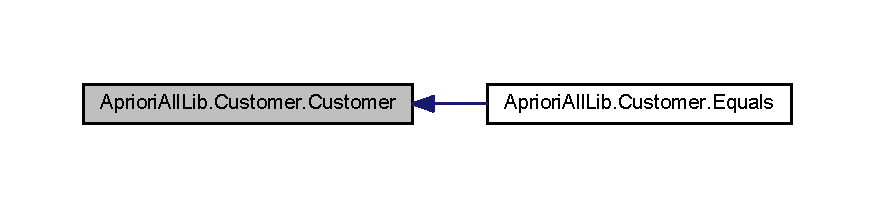
\includegraphics[width=350pt]{class_apriori_all_lib_1_1_customer_af02616d948989c7ff6161efc2488ecab_icgraph}
\end{center}
\end{figure}


\hypertarget{class_apriori_all_lib_1_1_customer_a168c8ef2fa0b53671ea51fa21d788f7e}{\index{Apriori\-All\-Lib\-::\-Customer@{Apriori\-All\-Lib\-::\-Customer}!Customer@{Customer}}
\index{Customer@{Customer}!AprioriAllLib::Customer@{Apriori\-All\-Lib\-::\-Customer}}
\subsubsection[{Customer}]{\setlength{\rightskip}{0pt plus 5cm}Apriori\-All\-Lib.\-Customer.\-Customer (
\begin{DoxyParamCaption}
\item[{params {\bf Transaction}\mbox{[}$\,$\mbox{]}}]{transactions}
\end{DoxyParamCaption}
)}}\label{class_apriori_all_lib_1_1_customer_a168c8ef2fa0b53671ea51fa21d788f7e}


Constructor 


\begin{DoxyParams}{Parameters}
{\em transactions} & Array of transactions of this client\\
\hline
\end{DoxyParams}

\begin{DoxyCode}
                                                           \{
            \hyperlink{class_apriori_all_lib_1_1_customer_a5bf3b782d5e9c582e3f395834b7bddad}{Transactions} = \textcolor{keyword}{new} List<Transaction>();
            \textcolor{keywordflow}{foreach} (Transaction t \textcolor{keywordflow}{in} transactions)
                \hyperlink{class_apriori_all_lib_1_1_customer_a5bf3b782d5e9c582e3f395834b7bddad}{Transactions}.Add(t);
        \}
\end{DoxyCode}
\hypertarget{class_apriori_all_lib_1_1_customer_a8a0e52125e85fae2662fa7edb756cedd}{\index{Apriori\-All\-Lib\-::\-Customer@{Apriori\-All\-Lib\-::\-Customer}!Customer@{Customer}}
\index{Customer@{Customer}!AprioriAllLib::Customer@{Apriori\-All\-Lib\-::\-Customer}}
\subsubsection[{Customer}]{\setlength{\rightskip}{0pt plus 5cm}Apriori\-All\-Lib.\-Customer.\-Customer (
\begin{DoxyParamCaption}
\item[{params int}]{values\-Array\mbox{[}$\,$\mbox{]}\mbox{[}$\,$\mbox{]}}
\end{DoxyParamCaption}
)}}\label{class_apriori_all_lib_1_1_customer_a8a0e52125e85fae2662fa7edb756cedd}


Constructor 


\begin{DoxyParams}{Parameters}
{\em values\-Array} & Two-\/dimensional array of integer values of items in transactions of this client\\
\hline
\end{DoxyParams}

\begin{DoxyCode}
                                                    \{
            \hyperlink{class_apriori_all_lib_1_1_customer_a5bf3b782d5e9c582e3f395834b7bddad}{Transactions} = \textcolor{keyword}{new} List<Transaction>();
            \textcolor{keywordflow}{foreach} (\textcolor{keywordtype}{int}[] values \textcolor{keywordflow}{in} valuesArray)
                \hyperlink{class_apriori_all_lib_1_1_customer_a5bf3b782d5e9c582e3f395834b7bddad}{Transactions}.Add(\textcolor{keyword}{new} Transaction(values));
        \}
\end{DoxyCode}


\subsection{Member Function Documentation}
\hypertarget{class_apriori_all_lib_1_1_customer_a8036f14573c62b0e4785e7157a1f547b}{\index{Apriori\-All\-Lib\-::\-Customer@{Apriori\-All\-Lib\-::\-Customer}!Equals@{Equals}}
\index{Equals@{Equals}!AprioriAllLib::Customer@{Apriori\-All\-Lib\-::\-Customer}}
\subsubsection[{Equals}]{\setlength{\rightskip}{0pt plus 5cm}override bool Apriori\-All\-Lib.\-Customer.\-Equals (
\begin{DoxyParamCaption}
\item[{object}]{obj}
\end{DoxyParamCaption}
)}}\label{class_apriori_all_lib_1_1_customer_a8036f14573c62b0e4785e7157a1f547b}

\begin{DoxyCode}
                                                \{
            \textcolor{keywordflow}{if} (obj.GetType().Equals(typeof(\hyperlink{class_apriori_all_lib_1_1_customer_af02616d948989c7ff6161efc2488ecab}{Customer})) && \hyperlink{class_apriori_all_lib_1_1_customer_a5bf3b782d5e9c582e3f395834b7bddad}{Transactions}
      .Count == ((\hyperlink{class_apriori_all_lib_1_1_customer_af02616d948989c7ff6161efc2488ecab}{Customer})obj).Transactions.Count
                    && Enumerable.SequenceEqual(\hyperlink{class_apriori_all_lib_1_1_customer_a5bf3b782d5e9c582e3f395834b7bddad}{Transactions}, ((
      \hyperlink{class_apriori_all_lib_1_1_customer_af02616d948989c7ff6161efc2488ecab}{Customer})obj).\hyperlink{class_apriori_all_lib_1_1_customer_a5bf3b782d5e9c582e3f395834b7bddad}{Transactions}))
                \textcolor{keywordflow}{return} \textcolor{keyword}{true};
            \textcolor{keywordflow}{return} \textcolor{keyword}{false};
            \textcolor{comment}{//return base.Equals(obj);}
        \}
\end{DoxyCode}


Here is the call graph for this function\-:\nopagebreak
\begin{figure}[H]
\begin{center}
\leavevmode
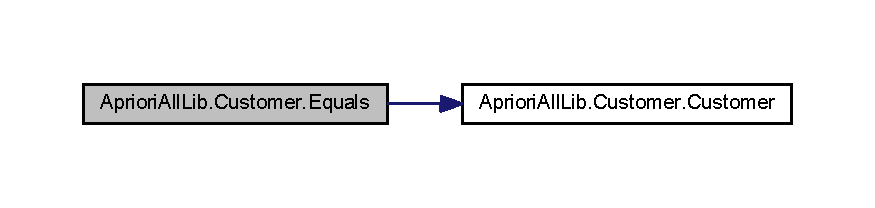
\includegraphics[width=350pt]{class_apriori_all_lib_1_1_customer_a8036f14573c62b0e4785e7157a1f547b_cgraph}
\end{center}
\end{figure}


\hypertarget{class_apriori_all_lib_1_1_customer_a311c3424f3f1207afe9b883cc41cae60}{\index{Apriori\-All\-Lib\-::\-Customer@{Apriori\-All\-Lib\-::\-Customer}!To\-String@{To\-String}}
\index{To\-String@{To\-String}!AprioriAllLib::Customer@{Apriori\-All\-Lib\-::\-Customer}}
\subsubsection[{To\-String}]{\setlength{\rightskip}{0pt plus 5cm}override string Apriori\-All\-Lib.\-Customer.\-To\-String (
\begin{DoxyParamCaption}
{}
\end{DoxyParamCaption}
)}}\label{class_apriori_all_lib_1_1_customer_a311c3424f3f1207afe9b883cc41cae60}


Prints the content of client transactions 

\begin{DoxyReturn}{Returns}
String of values of transaction items
\end{DoxyReturn}

\begin{DoxyCode}
                                          \{
            \textcolor{keywordtype}{string} itemsStr = \textcolor{keywordtype}{string}.Join(\textcolor{stringliteral}{","}, \hyperlink{class_apriori_all_lib_1_1_customer_a5bf3b782d5e9c582e3f395834b7bddad}{Transactions}.Select(
      x => x.ToString()).ToArray());
            \textcolor{keywordflow}{return} String.Format(\textcolor{stringliteral}{"\{0\}"}, itemsStr);
        \}
\end{DoxyCode}


\subsection{Member Data Documentation}
\hypertarget{class_apriori_all_lib_1_1_customer_a5bf3b782d5e9c582e3f395834b7bddad}{\index{Apriori\-All\-Lib\-::\-Customer@{Apriori\-All\-Lib\-::\-Customer}!Transactions@{Transactions}}
\index{Transactions@{Transactions}!AprioriAllLib::Customer@{Apriori\-All\-Lib\-::\-Customer}}
\subsubsection[{Transactions}]{\setlength{\rightskip}{0pt plus 5cm}List$<${\bf Transaction}$>$ Apriori\-All\-Lib.\-Customer.\-Transactions}}\label{class_apriori_all_lib_1_1_customer_a5bf3b782d5e9c582e3f395834b7bddad}


List of transactions 



The documentation for this class was generated from the following file\-:\begin{DoxyCompactItemize}
\item 
D\-:/\-Projects/\-Csharp/\-Mi\-N\-I\-\_\-\-Apriori\-All/\-Apriori\-All\-Lib/\hyperlink{_customer_8cs}{Customer.\-cs}\end{DoxyCompactItemize}

\hypertarget{class_apriori_all_lib_1_1_customer_list}{\section{Apriori\-All\-Lib.\-Customer\-List Class Reference}
\label{class_apriori_all_lib_1_1_customer_list}\index{Apriori\-All\-Lib.\-Customer\-List@{Apriori\-All\-Lib.\-Customer\-List}}
}


Class that represents a total set of customers  


\subsection*{Public Member Functions}
\begin{DoxyCompactItemize}
\item 
\hyperlink{class_apriori_all_lib_1_1_customer_list_abaf21c0d33a87db3cf61e0c0741a6d44}{Customer\-List} ()
\begin{DoxyCompactList}\small\item\em Constructor \end{DoxyCompactList}\item 
override string \hyperlink{class_apriori_all_lib_1_1_customer_list_a8f3853844dc1e35424a54e706014f8d7}{To\-String} ()
\begin{DoxyCompactList}\small\item\em String representation of this class \end{DoxyCompactList}\end{DoxyCompactItemize}
\subsection*{Public Attributes}
\begin{DoxyCompactItemize}
\item 
List$<$ \hyperlink{class_apriori_all_lib_1_1_customer}{Customer} $>$ \hyperlink{class_apriori_all_lib_1_1_customer_list_a4fd2a16a984844e61ffc60b327e6534a}{Customers}
\begin{DoxyCompactList}\small\item\em List of Customers \end{DoxyCompactList}\end{DoxyCompactItemize}


\subsection{Detailed Description}
Class that represents a total set of customers 



\subsection{Constructor \& Destructor Documentation}
\hypertarget{class_apriori_all_lib_1_1_customer_list_abaf21c0d33a87db3cf61e0c0741a6d44}{\index{Apriori\-All\-Lib\-::\-Customer\-List@{Apriori\-All\-Lib\-::\-Customer\-List}!Customer\-List@{Customer\-List}}
\index{Customer\-List@{Customer\-List}!AprioriAllLib::CustomerList@{Apriori\-All\-Lib\-::\-Customer\-List}}
\subsubsection[{Customer\-List}]{\setlength{\rightskip}{0pt plus 5cm}Apriori\-All\-Lib.\-Customer\-List.\-Customer\-List (
\begin{DoxyParamCaption}
{}
\end{DoxyParamCaption}
)}}\label{class_apriori_all_lib_1_1_customer_list_abaf21c0d33a87db3cf61e0c0741a6d44}


Constructor 


\begin{DoxyCode}
                              \{
            \hyperlink{class_apriori_all_lib_1_1_customer_list_a4fd2a16a984844e61ffc60b327e6534a}{Customers} = \textcolor{keyword}{new} List<Customer>();
        \}
\end{DoxyCode}


\subsection{Member Function Documentation}
\hypertarget{class_apriori_all_lib_1_1_customer_list_a8f3853844dc1e35424a54e706014f8d7}{\index{Apriori\-All\-Lib\-::\-Customer\-List@{Apriori\-All\-Lib\-::\-Customer\-List}!To\-String@{To\-String}}
\index{To\-String@{To\-String}!AprioriAllLib::CustomerList@{Apriori\-All\-Lib\-::\-Customer\-List}}
\subsubsection[{To\-String}]{\setlength{\rightskip}{0pt plus 5cm}override string Apriori\-All\-Lib.\-Customer\-List.\-To\-String (
\begin{DoxyParamCaption}
{}
\end{DoxyParamCaption}
)}}\label{class_apriori_all_lib_1_1_customer_list_a8f3853844dc1e35424a54e706014f8d7}


String representation of this class 

\begin{DoxyReturn}{Returns}
String representation
\end{DoxyReturn}

\begin{DoxyCode}
                                          \{
            \textcolor{keywordtype}{string} itemsStr = \textcolor{keywordtype}{string}.Join(\textcolor{stringliteral}{"; "}, \hyperlink{class_apriori_all_lib_1_1_customer_list_a4fd2a16a984844e61ffc60b327e6534a}{Customers}.Select(x => 
      x.ToString()).ToArray());
            \textcolor{keywordflow}{return} String.Format(\textcolor{stringliteral}{"CuLst[ \{0\} ]"}, itemsStr);
        \}
\end{DoxyCode}


\subsection{Member Data Documentation}
\hypertarget{class_apriori_all_lib_1_1_customer_list_a4fd2a16a984844e61ffc60b327e6534a}{\index{Apriori\-All\-Lib\-::\-Customer\-List@{Apriori\-All\-Lib\-::\-Customer\-List}!Customers@{Customers}}
\index{Customers@{Customers}!AprioriAllLib::CustomerList@{Apriori\-All\-Lib\-::\-Customer\-List}}
\subsubsection[{Customers}]{\setlength{\rightskip}{0pt plus 5cm}List$<${\bf Customer}$>$ Apriori\-All\-Lib.\-Customer\-List.\-Customers}}\label{class_apriori_all_lib_1_1_customer_list_a4fd2a16a984844e61ffc60b327e6534a}


List of Customers 



The documentation for this class was generated from the following file\-:\begin{DoxyCompactItemize}
\item 
D\-:/\-Projects/\-Csharp/\-Mi\-N\-I\-\_\-\-Apriori\-All/\-Apriori\-All\-Lib/\hyperlink{_customer_list_8cs}{Customer\-List.\-cs}\end{DoxyCompactItemize}

\hypertarget{class_apriori_all_lib_1_1_item}{\section{Apriori\-All\-Lib.\-Item Class Reference}
\label{class_apriori_all_lib_1_1_item}\index{Apriori\-All\-Lib.\-Item@{Apriori\-All\-Lib.\-Item}}
}


Single item of a transaction.  




Inheritance diagram for Apriori\-All\-Lib.\-Item\-:\nopagebreak
\begin{figure}[H]
\begin{center}
\leavevmode
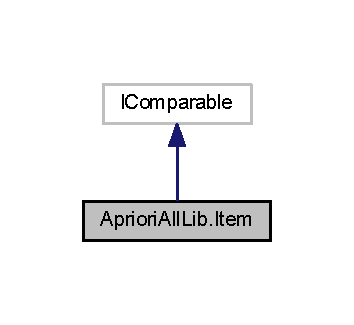
\includegraphics[width=170pt]{class_apriori_all_lib_1_1_item__inherit__graph}
\end{center}
\end{figure}


Collaboration diagram for Apriori\-All\-Lib.\-Item\-:\nopagebreak
\begin{figure}[H]
\begin{center}
\leavevmode
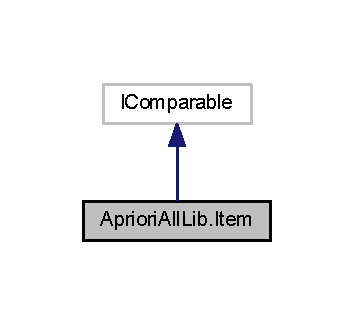
\includegraphics[width=170pt]{class_apriori_all_lib_1_1_item__coll__graph}
\end{center}
\end{figure}
\subsection*{Public Member Functions}
\begin{DoxyCompactItemize}
\item 
\hyperlink{class_apriori_all_lib_1_1_item_aed218e4e6b27b6ac780be54f6f483d59}{Item} (int value)
\begin{DoxyCompactList}\small\item\em Constructor \end{DoxyCompactList}\item 
int \hyperlink{class_apriori_all_lib_1_1_item_a0b0e9bbfeea95abed90935db84beb999}{Compare\-To} (object obj)
\item 
override string \hyperlink{class_apriori_all_lib_1_1_item_a020b36119d00b63670da5688967dc147}{To\-String} ()
\begin{DoxyCompactList}\small\item\em String representation of this class \end{DoxyCompactList}\item 
override bool \hyperlink{class_apriori_all_lib_1_1_item_a69489ac60415029faf0dc3e7dc926e62}{Equals} (object obj)
\end{DoxyCompactItemize}
\subsection*{Public Attributes}
\begin{DoxyCompactItemize}
\item 
int \hyperlink{class_apriori_all_lib_1_1_item_ab54b4b9529a99f74048264c3ed2ab6bd}{Value}
\begin{DoxyCompactList}\small\item\em Integer value (id) of the item \end{DoxyCompactList}\end{DoxyCompactItemize}


\subsection{Detailed Description}
Single item of a transaction. 



\subsection{Constructor \& Destructor Documentation}
\hypertarget{class_apriori_all_lib_1_1_item_aed218e4e6b27b6ac780be54f6f483d59}{\index{Apriori\-All\-Lib\-::\-Item@{Apriori\-All\-Lib\-::\-Item}!Item@{Item}}
\index{Item@{Item}!AprioriAllLib::Item@{Apriori\-All\-Lib\-::\-Item}}
\subsubsection[{Item}]{\setlength{\rightskip}{0pt plus 5cm}Apriori\-All\-Lib.\-Item.\-Item (
\begin{DoxyParamCaption}
\item[{int}]{value}
\end{DoxyParamCaption}
)}}\label{class_apriori_all_lib_1_1_item_aed218e4e6b27b6ac780be54f6f483d59}


Constructor 


\begin{DoxyParams}{Parameters}
{\em value} & Value of the item\\
\hline
\end{DoxyParams}

\begin{DoxyCode}
                               \{
            this.\hyperlink{class_apriori_all_lib_1_1_item_ab54b4b9529a99f74048264c3ed2ab6bd}{Value} = value;
        \}
\end{DoxyCode}


Here is the caller graph for this function\-:\nopagebreak
\begin{figure}[H]
\begin{center}
\leavevmode
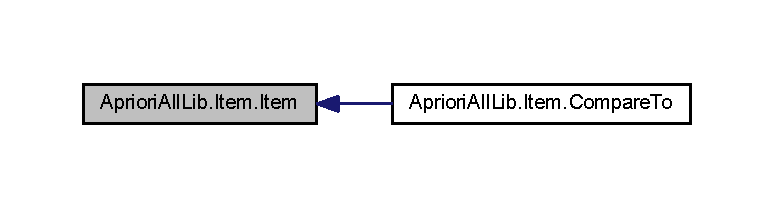
\includegraphics[width=350pt]{class_apriori_all_lib_1_1_item_aed218e4e6b27b6ac780be54f6f483d59_icgraph}
\end{center}
\end{figure}




\subsection{Member Function Documentation}
\hypertarget{class_apriori_all_lib_1_1_item_a0b0e9bbfeea95abed90935db84beb999}{\index{Apriori\-All\-Lib\-::\-Item@{Apriori\-All\-Lib\-::\-Item}!Compare\-To@{Compare\-To}}
\index{Compare\-To@{Compare\-To}!AprioriAllLib::Item@{Apriori\-All\-Lib\-::\-Item}}
\subsubsection[{Compare\-To}]{\setlength{\rightskip}{0pt plus 5cm}int Apriori\-All\-Lib.\-Item.\-Compare\-To (
\begin{DoxyParamCaption}
\item[{object}]{obj}
\end{DoxyParamCaption}
)}}\label{class_apriori_all_lib_1_1_item_a0b0e9bbfeea95abed90935db84beb999}

\begin{DoxyCode}
                                         \{
            \textcolor{keywordflow}{return} ((\hyperlink{class_apriori_all_lib_1_1_item_aed218e4e6b27b6ac780be54f6f483d59}{Item})obj).Value == this.\hyperlink{class_apriori_all_lib_1_1_item_ab54b4b9529a99f74048264c3ed2ab6bd}{Value} ? 0 : (((\hyperlink{class_apriori_all_lib_1_1_item_aed218e4e6b27b6ac780be54f6f483d59}{Item})
      obj).Value > this.\hyperlink{class_apriori_all_lib_1_1_item_ab54b4b9529a99f74048264c3ed2ab6bd}{Value} ? -1 : 1);
        \}
\end{DoxyCode}


Here is the call graph for this function\-:\nopagebreak
\begin{figure}[H]
\begin{center}
\leavevmode
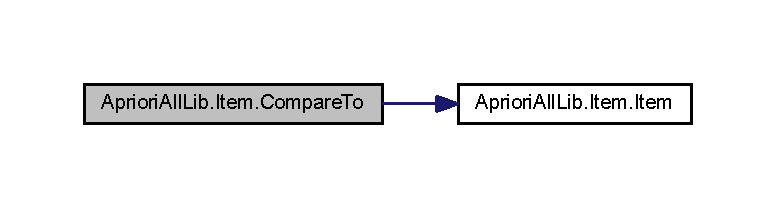
\includegraphics[width=350pt]{class_apriori_all_lib_1_1_item_a0b0e9bbfeea95abed90935db84beb999_cgraph}
\end{center}
\end{figure}


\hypertarget{class_apriori_all_lib_1_1_item_a69489ac60415029faf0dc3e7dc926e62}{\index{Apriori\-All\-Lib\-::\-Item@{Apriori\-All\-Lib\-::\-Item}!Equals@{Equals}}
\index{Equals@{Equals}!AprioriAllLib::Item@{Apriori\-All\-Lib\-::\-Item}}
\subsubsection[{Equals}]{\setlength{\rightskip}{0pt plus 5cm}override bool Apriori\-All\-Lib.\-Item.\-Equals (
\begin{DoxyParamCaption}
\item[{object}]{obj}
\end{DoxyParamCaption}
)}}\label{class_apriori_all_lib_1_1_item_a69489ac60415029faf0dc3e7dc926e62}

\begin{DoxyCode}
                                                \{
            \textcolor{keywordflow}{if} (typeof(\hyperlink{class_apriori_all_lib_1_1_item_aed218e4e6b27b6ac780be54f6f483d59}{Item}).\hyperlink{class_apriori_all_lib_1_1_item_a69489ac60415029faf0dc3e7dc926e62}{Equals}(obj.GetType()) && ((\hyperlink{class_apriori_all_lib_1_1_item_aed218e4e6b27b6ac780be54f6f483d59}{Item})obj)
      .\hyperlink{class_apriori_all_lib_1_1_item_ab54b4b9529a99f74048264c3ed2ab6bd}{Value} == \hyperlink{class_apriori_all_lib_1_1_item_ab54b4b9529a99f74048264c3ed2ab6bd}{Value})
                \textcolor{keywordflow}{return} \textcolor{keyword}{true};
            \textcolor{keywordflow}{return} \textcolor{keyword}{false};
        \}
\end{DoxyCode}


Here is the caller graph for this function\-:
\nopagebreak
\begin{figure}[H]
\begin{center}
\leavevmode
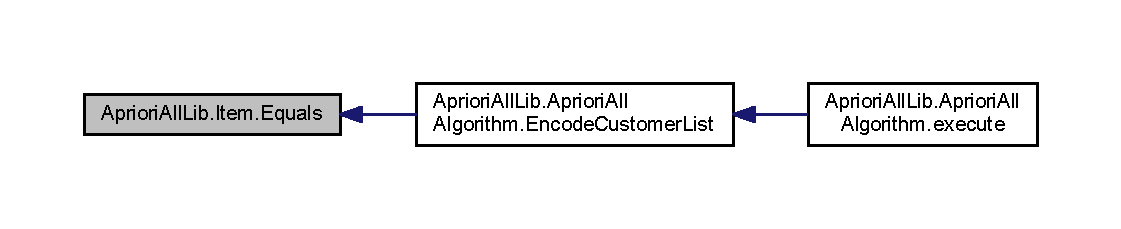
\includegraphics[width=350pt]{class_apriori_all_lib_1_1_item_a69489ac60415029faf0dc3e7dc926e62_icgraph}
\end{center}
\end{figure}


\hypertarget{class_apriori_all_lib_1_1_item_a020b36119d00b63670da5688967dc147}{\index{Apriori\-All\-Lib\-::\-Item@{Apriori\-All\-Lib\-::\-Item}!To\-String@{To\-String}}
\index{To\-String@{To\-String}!AprioriAllLib::Item@{Apriori\-All\-Lib\-::\-Item}}
\subsubsection[{To\-String}]{\setlength{\rightskip}{0pt plus 5cm}override string Apriori\-All\-Lib.\-Item.\-To\-String (
\begin{DoxyParamCaption}
{}
\end{DoxyParamCaption}
)}}\label{class_apriori_all_lib_1_1_item_a020b36119d00b63670da5688967dc147}


String representation of this class 

\begin{DoxyReturn}{Returns}
String representation
\end{DoxyReturn}

\begin{DoxyCode}
                                          \{
            \textcolor{keywordflow}{return} String.Format(\textcolor{stringliteral}{"\{0\}"}, \hyperlink{class_apriori_all_lib_1_1_item_ab54b4b9529a99f74048264c3ed2ab6bd}{Value});
        \}
\end{DoxyCode}


\subsection{Member Data Documentation}
\hypertarget{class_apriori_all_lib_1_1_item_ab54b4b9529a99f74048264c3ed2ab6bd}{\index{Apriori\-All\-Lib\-::\-Item@{Apriori\-All\-Lib\-::\-Item}!Value@{Value}}
\index{Value@{Value}!AprioriAllLib::Item@{Apriori\-All\-Lib\-::\-Item}}
\subsubsection[{Value}]{\setlength{\rightskip}{0pt plus 5cm}int Apriori\-All\-Lib.\-Item.\-Value}}\label{class_apriori_all_lib_1_1_item_ab54b4b9529a99f74048264c3ed2ab6bd}


Integer value (id) of the item 



The documentation for this class was generated from the following file\-:\begin{DoxyCompactItemize}
\item 
D\-:/\-Projects/\-Csharp/\-Mi\-N\-I\-\_\-\-Apriori\-All/\-Apriori\-All\-Lib/\hyperlink{_item_8cs}{Item.\-cs}\end{DoxyCompactItemize}

\hypertarget{class_apriori_all_lib_1_1_litemset}{\section{Apriori\-All\-Lib.\-Litemset Class Reference}
\label{class_apriori_all_lib_1_1_litemset}\index{Apriori\-All\-Lib.\-Litemset@{Apriori\-All\-Lib.\-Litemset}}
}


Class that represents a litemset (1-\/itemset)  


Inheritance diagram for Apriori\-All\-Lib.\-Litemset\-:\begin{figure}[H]
\begin{center}
\leavevmode
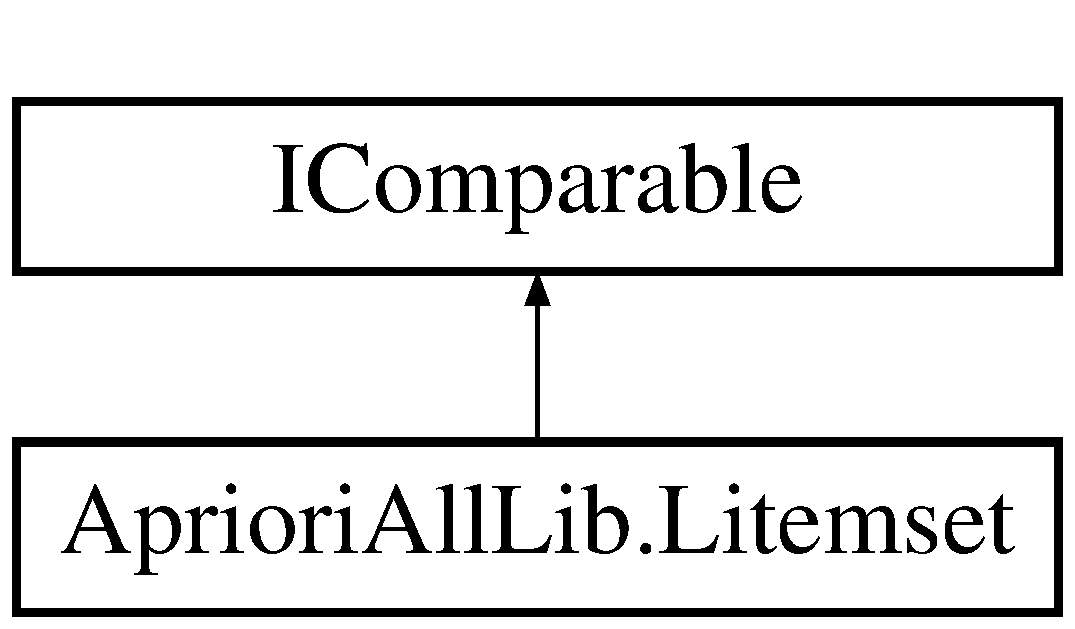
\includegraphics[height=2.000000cm]{class_apriori_all_lib_1_1_litemset}
\end{center}
\end{figure}
\subsection*{Public Member Functions}
\begin{DoxyCompactItemize}
\item 
\hyperlink{class_apriori_all_lib_1_1_litemset_af490087265e5b6389f19ce52775e6f35}{Litemset} ()
\begin{DoxyCompactList}\small\item\em Constructor \end{DoxyCompactList}\item 
\hyperlink{class_apriori_all_lib_1_1_litemset_a332a50f3e028dafcf393addcca5f3fb3}{Litemset} (List$<$ \hyperlink{class_apriori_all_lib_1_1_item}{Item} $>$ items)
\begin{DoxyCompactList}\small\item\em Constructor \end{DoxyCompactList}\item 
\hyperlink{class_apriori_all_lib_1_1_litemset_a2f9611a4cc391651629df60ea2e2f3e9}{Litemset} (int support, params int\mbox{[}$\,$\mbox{]} values)
\begin{DoxyCompactList}\small\item\em Constructor \end{DoxyCompactList}\item 
\hypertarget{class_apriori_all_lib_1_1_litemset_afcbe1c14c38d2638cb48ed9305de5a4e}{int {\bfseries Compare\-To} (object obj)}\label{class_apriori_all_lib_1_1_litemset_afcbe1c14c38d2638cb48ed9305de5a4e}

\item 
override string \hyperlink{class_apriori_all_lib_1_1_litemset_a512b70867120363edcd1178cec1c31f9}{To\-String} ()
\begin{DoxyCompactList}\small\item\em String representation of this class \end{DoxyCompactList}\end{DoxyCompactItemize}
\subsection*{Public Attributes}
\begin{DoxyCompactItemize}
\item 
int \hyperlink{class_apriori_all_lib_1_1_litemset_a9f37ba3b3423bc7a1619493132dbc3e2}{Support}
\begin{DoxyCompactList}\small\item\em Support of this litemset \end{DoxyCompactList}\item 
List$<$ int $>$ \hyperlink{class_apriori_all_lib_1_1_litemset_a74c9ee16b225268e66ee77d69142bc1a}{I\-Ds}
\begin{DoxyCompactList}\small\item\em List of I\-Ds of clients that support this litemset \end{DoxyCompactList}\item 
List$<$ \hyperlink{class_apriori_all_lib_1_1_item}{Item} $>$ \hyperlink{class_apriori_all_lib_1_1_litemset_aef38d5fccb4e45867abf5838ab8a68fa}{Items}
\begin{DoxyCompactList}\small\item\em List of items that this litemset contains \end{DoxyCompactList}\end{DoxyCompactItemize}


\subsection{Detailed Description}
Class that represents a litemset (1-\/itemset) 



\subsection{Constructor \& Destructor Documentation}
\hypertarget{class_apriori_all_lib_1_1_litemset_af490087265e5b6389f19ce52775e6f35}{\index{Apriori\-All\-Lib\-::\-Litemset@{Apriori\-All\-Lib\-::\-Litemset}!Litemset@{Litemset}}
\index{Litemset@{Litemset}!AprioriAllLib::Litemset@{Apriori\-All\-Lib\-::\-Litemset}}
\subsubsection[{Litemset}]{\setlength{\rightskip}{0pt plus 5cm}Apriori\-All\-Lib.\-Litemset.\-Litemset (
\begin{DoxyParamCaption}
{}
\end{DoxyParamCaption}
)}}\label{class_apriori_all_lib_1_1_litemset_af490087265e5b6389f19ce52775e6f35}


Constructor 


\begin{DoxyCode}
                          \{
        \}
\end{DoxyCode}
\hypertarget{class_apriori_all_lib_1_1_litemset_a332a50f3e028dafcf393addcca5f3fb3}{\index{Apriori\-All\-Lib\-::\-Litemset@{Apriori\-All\-Lib\-::\-Litemset}!Litemset@{Litemset}}
\index{Litemset@{Litemset}!AprioriAllLib::Litemset@{Apriori\-All\-Lib\-::\-Litemset}}
\subsubsection[{Litemset}]{\setlength{\rightskip}{0pt plus 5cm}Apriori\-All\-Lib.\-Litemset.\-Litemset (
\begin{DoxyParamCaption}
\item[{List$<$ {\bf Item} $>$}]{items}
\end{DoxyParamCaption}
)}}\label{class_apriori_all_lib_1_1_litemset_a332a50f3e028dafcf393addcca5f3fb3}


Constructor 


\begin{DoxyParams}{Parameters}
{\em items} & List of items\\
\hline
\end{DoxyParams}

\begin{DoxyCode}
                                          \{
            \hyperlink{class_apriori_all_lib_1_1_litemset_aef38d5fccb4e45867abf5838ab8a68fa}{Items} = items;
            \hyperlink{class_apriori_all_lib_1_1_litemset_a74c9ee16b225268e66ee77d69142bc1a}{IDs} = \textcolor{keyword}{new} List<int>();
        \}
\end{DoxyCode}
\hypertarget{class_apriori_all_lib_1_1_litemset_a2f9611a4cc391651629df60ea2e2f3e9}{\index{Apriori\-All\-Lib\-::\-Litemset@{Apriori\-All\-Lib\-::\-Litemset}!Litemset@{Litemset}}
\index{Litemset@{Litemset}!AprioriAllLib::Litemset@{Apriori\-All\-Lib\-::\-Litemset}}
\subsubsection[{Litemset}]{\setlength{\rightskip}{0pt plus 5cm}Apriori\-All\-Lib.\-Litemset.\-Litemset (
\begin{DoxyParamCaption}
\item[{int}]{support, }
\item[{params int\mbox{[}$\,$\mbox{]}}]{values}
\end{DoxyParamCaption}
)}}\label{class_apriori_all_lib_1_1_litemset_a2f9611a4cc391651629df60ea2e2f3e9}


Constructor 


\begin{DoxyParams}{Parameters}
{\em support} & Support\\
\hline
{\em values} & Values of items\\
\hline
\end{DoxyParams}

\begin{DoxyCode}
                                                          \{
            \textcolor{keywordflow}{if} (values == null)
                \textcolor{keywordflow}{throw} \textcolor{keyword}{new} ArgumentNullException(\textcolor{stringliteral}{"values"}, \textcolor{stringliteral}{"values is null."});
            \hyperlink{class_apriori_all_lib_1_1_litemset_a9f37ba3b3423bc7a1619493132dbc3e2}{Support} = support;
            \hyperlink{class_apriori_all_lib_1_1_litemset_aef38d5fccb4e45867abf5838ab8a68fa}{Items} = \textcolor{keyword}{new} List<Item>();
            \textcolor{keywordflow}{foreach} (\textcolor{keywordtype}{int} value \textcolor{keywordflow}{in} values)
                \hyperlink{class_apriori_all_lib_1_1_litemset_aef38d5fccb4e45867abf5838ab8a68fa}{Items}.Add(\textcolor{keyword}{new} Item(value));
        \}
\end{DoxyCode}


\subsection{Member Function Documentation}
\hypertarget{class_apriori_all_lib_1_1_litemset_a512b70867120363edcd1178cec1c31f9}{\index{Apriori\-All\-Lib\-::\-Litemset@{Apriori\-All\-Lib\-::\-Litemset}!To\-String@{To\-String}}
\index{To\-String@{To\-String}!AprioriAllLib::Litemset@{Apriori\-All\-Lib\-::\-Litemset}}
\subsubsection[{To\-String}]{\setlength{\rightskip}{0pt plus 5cm}override string Apriori\-All\-Lib.\-Litemset.\-To\-String (
\begin{DoxyParamCaption}
{}
\end{DoxyParamCaption}
)}}\label{class_apriori_all_lib_1_1_litemset_a512b70867120363edcd1178cec1c31f9}


String representation of this class 

\begin{DoxyReturn}{Returns}
String representation
\end{DoxyReturn}

\begin{DoxyCode}
                                          \{
            \textcolor{keywordtype}{string} itemsStr = \textcolor{keywordtype}{string}.Join(\textcolor{stringliteral}{","}, \hyperlink{class_apriori_all_lib_1_1_litemset_aef38d5fccb4e45867abf5838ab8a68fa}{Items}.Select(x => x.
      ToString()).ToArray());
            \textcolor{keywordflow}{return} String.Format(\textcolor{stringliteral}{"Lit(Supp=\{0\};\{1\})"}, \hyperlink{class_apriori_all_lib_1_1_litemset_a9f37ba3b3423bc7a1619493132dbc3e2}{Support}, itemsStr)
      ;
        \}
\end{DoxyCode}


\subsection{Member Data Documentation}
\hypertarget{class_apriori_all_lib_1_1_litemset_a74c9ee16b225268e66ee77d69142bc1a}{\index{Apriori\-All\-Lib\-::\-Litemset@{Apriori\-All\-Lib\-::\-Litemset}!I\-Ds@{I\-Ds}}
\index{I\-Ds@{I\-Ds}!AprioriAllLib::Litemset@{Apriori\-All\-Lib\-::\-Litemset}}
\subsubsection[{I\-Ds}]{\setlength{\rightskip}{0pt plus 5cm}List$<$int$>$ Apriori\-All\-Lib.\-Litemset.\-I\-Ds}}\label{class_apriori_all_lib_1_1_litemset_a74c9ee16b225268e66ee77d69142bc1a}


List of I\-Ds of clients that support this litemset 

\hypertarget{class_apriori_all_lib_1_1_litemset_aef38d5fccb4e45867abf5838ab8a68fa}{\index{Apriori\-All\-Lib\-::\-Litemset@{Apriori\-All\-Lib\-::\-Litemset}!Items@{Items}}
\index{Items@{Items}!AprioriAllLib::Litemset@{Apriori\-All\-Lib\-::\-Litemset}}
\subsubsection[{Items}]{\setlength{\rightskip}{0pt plus 5cm}List$<${\bf Item}$>$ Apriori\-All\-Lib.\-Litemset.\-Items}}\label{class_apriori_all_lib_1_1_litemset_aef38d5fccb4e45867abf5838ab8a68fa}


List of items that this litemset contains 

\hypertarget{class_apriori_all_lib_1_1_litemset_a9f37ba3b3423bc7a1619493132dbc3e2}{\index{Apriori\-All\-Lib\-::\-Litemset@{Apriori\-All\-Lib\-::\-Litemset}!Support@{Support}}
\index{Support@{Support}!AprioriAllLib::Litemset@{Apriori\-All\-Lib\-::\-Litemset}}
\subsubsection[{Support}]{\setlength{\rightskip}{0pt plus 5cm}int Apriori\-All\-Lib.\-Litemset.\-Support}}\label{class_apriori_all_lib_1_1_litemset_a9f37ba3b3423bc7a1619493132dbc3e2}


Support of this litemset 



The documentation for this class was generated from the following file\-:\begin{DoxyCompactItemize}
\item 
D\-:/\-Projects/\-Csharp/\-Mi\-N\-I\-\_\-\-Apriori\-All/\-Apriori\-All\-Lib/Litemset.\-cs\end{DoxyCompactItemize}

\hypertarget{class_apriori_all_lib_1_1_transaction}{\section{Apriori\-All\-Lib.\-Transaction Class Reference}
\label{class_apriori_all_lib_1_1_transaction}\index{Apriori\-All\-Lib.\-Transaction@{Apriori\-All\-Lib.\-Transaction}}
}


Single client's transaction having a list of items  


\subsection*{Public Member Functions}
\begin{DoxyCompactItemize}
\item 
\hyperlink{class_apriori_all_lib_1_1_transaction_adad35699bc55fcba5ee7ad28d34bdf53}{Transaction} ()
\begin{DoxyCompactList}\small\item\em Constructor \end{DoxyCompactList}\item 
\hyperlink{class_apriori_all_lib_1_1_transaction_a582a1d655d1c0d452a5e5f0b972688dd}{Transaction} (params int\mbox{[}$\,$\mbox{]} values)
\begin{DoxyCompactList}\small\item\em Constructor \end{DoxyCompactList}\item 
override string \hyperlink{class_apriori_all_lib_1_1_transaction_acee1a8846d87f949c63110f7e6eabfe0}{To\-String} ()
\begin{DoxyCompactList}\small\item\em Prints the content of transaction \end{DoxyCompactList}\end{DoxyCompactItemize}
\subsection*{Public Attributes}
\begin{DoxyCompactItemize}
\item 
\hypertarget{class_apriori_all_lib_1_1_transaction_a2ee6b2f74a842edb646ec8f99e5f7b8f}{List$<$ List$<$ \hyperlink{class_apriori_all_lib_1_1_item}{Item} $>$ $>$ {\bfseries Frequent\-Items}}\label{class_apriori_all_lib_1_1_transaction_a2ee6b2f74a842edb646ec8f99e5f7b8f}

\end{DoxyCompactItemize}
\subsection*{Properties}
\begin{DoxyCompactItemize}
\item 
List$<$ \hyperlink{class_apriori_all_lib_1_1_item}{Item} $>$ \hyperlink{class_apriori_all_lib_1_1_transaction_abb1fe3a28d74f8b1cd5f5ca2add6a043}{Items}\hspace{0.3cm}{\ttfamily  \mbox{[}get, set\mbox{]}}
\begin{DoxyCompactList}\small\item\em A list of items \end{DoxyCompactList}\end{DoxyCompactItemize}


\subsection{Detailed Description}
Single client's transaction having a list of items 



\subsection{Constructor \& Destructor Documentation}
\hypertarget{class_apriori_all_lib_1_1_transaction_adad35699bc55fcba5ee7ad28d34bdf53}{\index{Apriori\-All\-Lib\-::\-Transaction@{Apriori\-All\-Lib\-::\-Transaction}!Transaction@{Transaction}}
\index{Transaction@{Transaction}!AprioriAllLib::Transaction@{Apriori\-All\-Lib\-::\-Transaction}}
\subsubsection[{Transaction}]{\setlength{\rightskip}{0pt plus 5cm}Apriori\-All\-Lib.\-Transaction.\-Transaction (
\begin{DoxyParamCaption}
{}
\end{DoxyParamCaption}
)}}\label{class_apriori_all_lib_1_1_transaction_adad35699bc55fcba5ee7ad28d34bdf53}


Constructor 

\hypertarget{class_apriori_all_lib_1_1_transaction_a582a1d655d1c0d452a5e5f0b972688dd}{\index{Apriori\-All\-Lib\-::\-Transaction@{Apriori\-All\-Lib\-::\-Transaction}!Transaction@{Transaction}}
\index{Transaction@{Transaction}!AprioriAllLib::Transaction@{Apriori\-All\-Lib\-::\-Transaction}}
\subsubsection[{Transaction}]{\setlength{\rightskip}{0pt plus 5cm}Apriori\-All\-Lib.\-Transaction.\-Transaction (
\begin{DoxyParamCaption}
\item[{params int\mbox{[}$\,$\mbox{]}}]{values}
\end{DoxyParamCaption}
)}}\label{class_apriori_all_lib_1_1_transaction_a582a1d655d1c0d452a5e5f0b972688dd}


Constructor 


\begin{DoxyParams}{Parameters}
{\em values} & Array of integer values of items contained in this transaction\\
\hline
\end{DoxyParams}


\subsection{Member Function Documentation}
\hypertarget{class_apriori_all_lib_1_1_transaction_acee1a8846d87f949c63110f7e6eabfe0}{\index{Apriori\-All\-Lib\-::\-Transaction@{Apriori\-All\-Lib\-::\-Transaction}!To\-String@{To\-String}}
\index{To\-String@{To\-String}!AprioriAllLib::Transaction@{Apriori\-All\-Lib\-::\-Transaction}}
\subsubsection[{To\-String}]{\setlength{\rightskip}{0pt plus 5cm}override string Apriori\-All\-Lib.\-Transaction.\-To\-String (
\begin{DoxyParamCaption}
{}
\end{DoxyParamCaption}
)}}\label{class_apriori_all_lib_1_1_transaction_acee1a8846d87f949c63110f7e6eabfe0}


Prints the content of transaction 

\begin{DoxyReturn}{Returns}
String of values of transaction items
\end{DoxyReturn}


\subsection{Property Documentation}
\hypertarget{class_apriori_all_lib_1_1_transaction_abb1fe3a28d74f8b1cd5f5ca2add6a043}{\index{Apriori\-All\-Lib\-::\-Transaction@{Apriori\-All\-Lib\-::\-Transaction}!Items@{Items}}
\index{Items@{Items}!AprioriAllLib::Transaction@{Apriori\-All\-Lib\-::\-Transaction}}
\subsubsection[{Items}]{\setlength{\rightskip}{0pt plus 5cm}List$<${\bf Item}$>$ Apriori\-All\-Lib.\-Transaction.\-Items\hspace{0.3cm}{\ttfamily [get]}, {\ttfamily [set]}}}\label{class_apriori_all_lib_1_1_transaction_abb1fe3a28d74f8b1cd5f5ca2add6a043}


A list of items 



The documentation for this class was generated from the following file\-:\begin{DoxyCompactItemize}
\item 
C\-:/\-Users/\-Karolina/\-Desktop/\-Apriori -\/ Copy/\-Apriori\-All\-Lib/Transaction.\-cs\end{DoxyCompactItemize}

\hypertarget{class_apriori_all_lib_1_1_xml_reader}{\section{Apriori\-All\-Lib.\-Xml\-Reader Class Reference}
\label{class_apriori_all_lib_1_1_xml_reader}\index{Apriori\-All\-Lib.\-Xml\-Reader@{Apriori\-All\-Lib.\-Xml\-Reader}}
}


Class that reads data from xml client database and transforms them into classes  


\subsection*{Public Member Functions}
\begin{DoxyCompactItemize}
\item 
\hyperlink{class_apriori_all_lib_1_1_customer_list}{Customer\-List} \hyperlink{class_apriori_all_lib_1_1_xml_reader_ab7285c4d5cee31f7a1001f00f4eeff25}{Read\-From\-Xml\-File} (string filename)
\begin{DoxyCompactList}\small\item\em Reads from xml client database \end{DoxyCompactList}\end{DoxyCompactItemize}
\subsection*{Private Member Functions}
\begin{DoxyCompactItemize}
\item 
void \hyperlink{class_apriori_all_lib_1_1_xml_reader_a117782b010f24408af2a1308786b473a}{add\-Customer} (Xml\-Text\-Reader reader, \hyperlink{class_apriori_all_lib_1_1_customer_list}{Customer\-List} list)
\item 
void \hyperlink{class_apriori_all_lib_1_1_xml_reader_ad39b320cc29d31704fbaa7b121cbc3ba}{add\-Transaction} (Xml\-Text\-Reader reader, \hyperlink{class_apriori_all_lib_1_1_customer}{Customer} customer)
\item 
void \hyperlink{class_apriori_all_lib_1_1_xml_reader_a24244fe32b889d4f7a4f44a9aeb11779}{add\-Item} (Xml\-Text\-Reader reader, \hyperlink{class_apriori_all_lib_1_1_transaction}{Transaction} transaction)
\end{DoxyCompactItemize}


\subsection{Detailed Description}
Class that reads data from xml client database and transforms them into classes 



\subsection{Member Function Documentation}
\hypertarget{class_apriori_all_lib_1_1_xml_reader_a117782b010f24408af2a1308786b473a}{\index{Apriori\-All\-Lib\-::\-Xml\-Reader@{Apriori\-All\-Lib\-::\-Xml\-Reader}!add\-Customer@{add\-Customer}}
\index{add\-Customer@{add\-Customer}!AprioriAllLib::XmlReader@{Apriori\-All\-Lib\-::\-Xml\-Reader}}
\subsubsection[{add\-Customer}]{\setlength{\rightskip}{0pt plus 5cm}void Apriori\-All\-Lib.\-Xml\-Reader.\-add\-Customer (
\begin{DoxyParamCaption}
\item[{Xml\-Text\-Reader}]{reader, }
\item[{{\bf Customer\-List}}]{list}
\end{DoxyParamCaption}
)\hspace{0.3cm}{\ttfamily [private]}}}\label{class_apriori_all_lib_1_1_xml_reader_a117782b010f24408af2a1308786b473a}

\begin{DoxyCode}
        \{
            Customer customer = \textcolor{keyword}{new} Customer();
            list.Customers.Add(customer);

            \textcolor{keywordflow}{while} (reader.Read() && (reader.NodeType != XmlNodeType.EndElement 
      || reader.Name != \textcolor{stringliteral}{"Customer"}))
            \{
                \textcolor{keywordflow}{if} (reader.NodeType == XmlNodeType.Element && reader.Name == \textcolor{stringliteral}{"
      Transaction"})
                    \hyperlink{class_apriori_all_lib_1_1_xml_reader_ad39b320cc29d31704fbaa7b121cbc3ba}{addTransaction}(reader, customer);
            \}
        \}
\end{DoxyCode}


Here is the call graph for this function\-:
\nopagebreak
\begin{figure}[H]
\begin{center}
\leavevmode
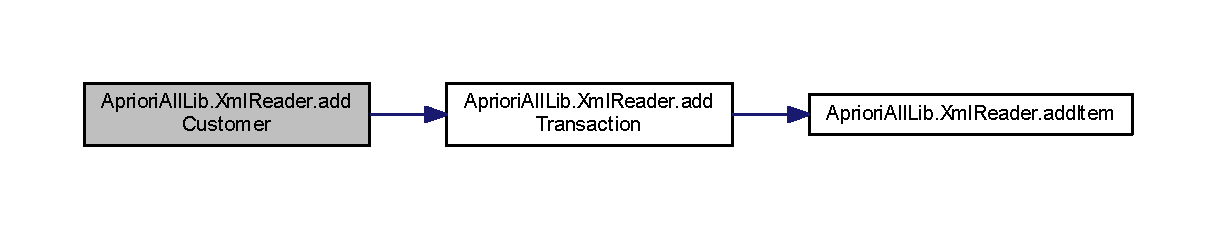
\includegraphics[width=350pt]{class_apriori_all_lib_1_1_xml_reader_a117782b010f24408af2a1308786b473a_cgraph}
\end{center}
\end{figure}




Here is the caller graph for this function\-:
\nopagebreak
\begin{figure}[H]
\begin{center}
\leavevmode
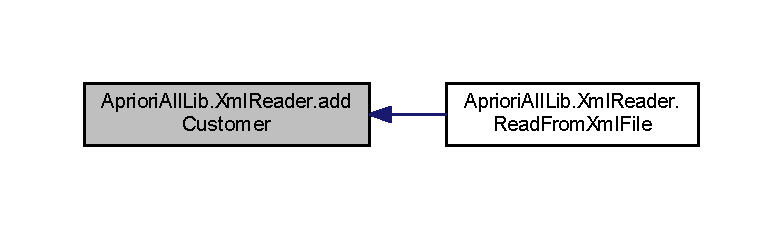
\includegraphics[width=350pt]{class_apriori_all_lib_1_1_xml_reader_a117782b010f24408af2a1308786b473a_icgraph}
\end{center}
\end{figure}


\hypertarget{class_apriori_all_lib_1_1_xml_reader_a24244fe32b889d4f7a4f44a9aeb11779}{\index{Apriori\-All\-Lib\-::\-Xml\-Reader@{Apriori\-All\-Lib\-::\-Xml\-Reader}!add\-Item@{add\-Item}}
\index{add\-Item@{add\-Item}!AprioriAllLib::XmlReader@{Apriori\-All\-Lib\-::\-Xml\-Reader}}
\subsubsection[{add\-Item}]{\setlength{\rightskip}{0pt plus 5cm}void Apriori\-All\-Lib.\-Xml\-Reader.\-add\-Item (
\begin{DoxyParamCaption}
\item[{Xml\-Text\-Reader}]{reader, }
\item[{{\bf Transaction}}]{transaction}
\end{DoxyParamCaption}
)\hspace{0.3cm}{\ttfamily [private]}}}\label{class_apriori_all_lib_1_1_xml_reader_a24244fe32b889d4f7a4f44a9aeb11779}

\begin{DoxyCode}
        \{
            \textcolor{keywordflow}{while} (reader.Read() && (reader.NodeType != XmlNodeType.EndElement)
       && reader.Name != \textcolor{stringliteral}{"Item"})
                \textcolor{keywordflow}{if} (reader.NodeType == XmlNodeType.Text && reader.HasValue)
                \{
                    transaction.Items.Add(\textcolor{keyword}{new} Item(\textcolor{keywordtype}{int}.Parse(reader.Value)));
                    \textcolor{comment}{//Console.WriteLine(reader.Value);}
                \}
        \}
\end{DoxyCode}


Here is the caller graph for this function\-:
\nopagebreak
\begin{figure}[H]
\begin{center}
\leavevmode
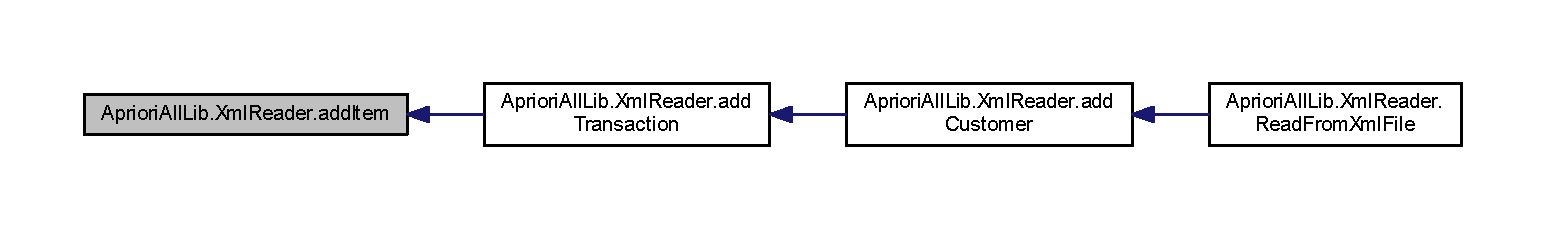
\includegraphics[width=350pt]{class_apriori_all_lib_1_1_xml_reader_a24244fe32b889d4f7a4f44a9aeb11779_icgraph}
\end{center}
\end{figure}


\hypertarget{class_apriori_all_lib_1_1_xml_reader_ad39b320cc29d31704fbaa7b121cbc3ba}{\index{Apriori\-All\-Lib\-::\-Xml\-Reader@{Apriori\-All\-Lib\-::\-Xml\-Reader}!add\-Transaction@{add\-Transaction}}
\index{add\-Transaction@{add\-Transaction}!AprioriAllLib::XmlReader@{Apriori\-All\-Lib\-::\-Xml\-Reader}}
\subsubsection[{add\-Transaction}]{\setlength{\rightskip}{0pt plus 5cm}void Apriori\-All\-Lib.\-Xml\-Reader.\-add\-Transaction (
\begin{DoxyParamCaption}
\item[{Xml\-Text\-Reader}]{reader, }
\item[{{\bf Customer}}]{customer}
\end{DoxyParamCaption}
)\hspace{0.3cm}{\ttfamily [private]}}}\label{class_apriori_all_lib_1_1_xml_reader_ad39b320cc29d31704fbaa7b121cbc3ba}

\begin{DoxyCode}
        \{
            Transaction transaction = \textcolor{keyword}{new} Transaction();
            customer.Transactions.Add(transaction);

            \textcolor{keywordflow}{while} (reader.Read() && (reader.NodeType != XmlNodeType.EndElement 
      || reader.Name != \textcolor{stringliteral}{"Transaction"}))
            \{
                \textcolor{keywordflow}{if} (reader.NodeType == XmlNodeType.Element && reader.Name == \textcolor{stringliteral}{"
      Item"})
                    \hyperlink{class_apriori_all_lib_1_1_xml_reader_a24244fe32b889d4f7a4f44a9aeb11779}{addItem}(reader, transaction);
            \}
        \}
\end{DoxyCode}


Here is the call graph for this function\-:
\nopagebreak
\begin{figure}[H]
\begin{center}
\leavevmode
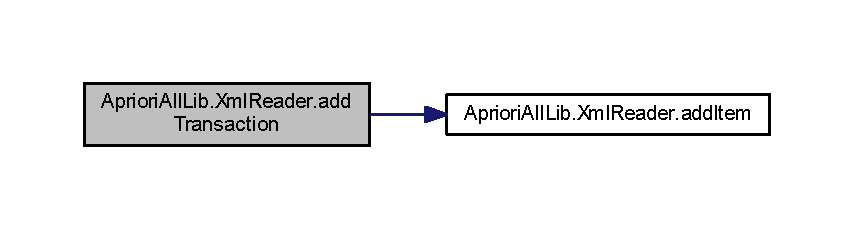
\includegraphics[width=350pt]{class_apriori_all_lib_1_1_xml_reader_ad39b320cc29d31704fbaa7b121cbc3ba_cgraph}
\end{center}
\end{figure}




Here is the caller graph for this function\-:
\nopagebreak
\begin{figure}[H]
\begin{center}
\leavevmode
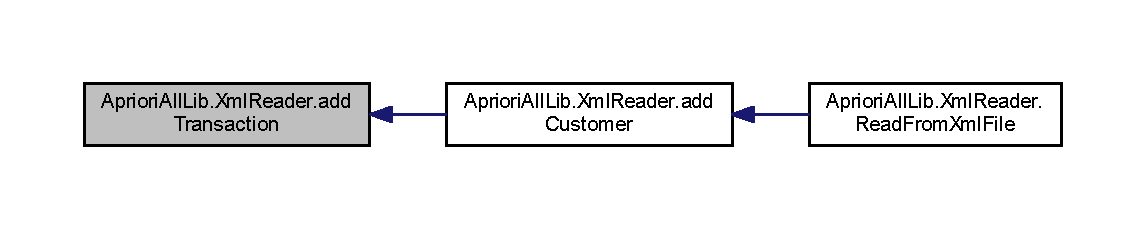
\includegraphics[width=350pt]{class_apriori_all_lib_1_1_xml_reader_ad39b320cc29d31704fbaa7b121cbc3ba_icgraph}
\end{center}
\end{figure}


\hypertarget{class_apriori_all_lib_1_1_xml_reader_ab7285c4d5cee31f7a1001f00f4eeff25}{\index{Apriori\-All\-Lib\-::\-Xml\-Reader@{Apriori\-All\-Lib\-::\-Xml\-Reader}!Read\-From\-Xml\-File@{Read\-From\-Xml\-File}}
\index{Read\-From\-Xml\-File@{Read\-From\-Xml\-File}!AprioriAllLib::XmlReader@{Apriori\-All\-Lib\-::\-Xml\-Reader}}
\subsubsection[{Read\-From\-Xml\-File}]{\setlength{\rightskip}{0pt plus 5cm}{\bf Customer\-List} Apriori\-All\-Lib.\-Xml\-Reader.\-Read\-From\-Xml\-File (
\begin{DoxyParamCaption}
\item[{string}]{filename}
\end{DoxyParamCaption}
)}}\label{class_apriori_all_lib_1_1_xml_reader_ab7285c4d5cee31f7a1001f00f4eeff25}


Reads from xml client database 


\begin{DoxyParams}{Parameters}
{\em filename} & String path of the database file\\
\hline
\end{DoxyParams}
\begin{DoxyReturn}{Returns}
Database transformed into a \hyperlink{class_apriori_all_lib_1_1_customer_list}{Customer\-List} object
\end{DoxyReturn}

\begin{DoxyCode}
        \{
            CustomerList list = \textcolor{keyword}{new} CustomerList();

            \textcolor{keywordflow}{try}
            \{
                XmlTextReader reader = \textcolor{keyword}{new} XmlTextReader(filename);
                \textcolor{keywordflow}{while} (reader.Read())
                \{
                    \textcolor{comment}{// Once we find the Clients tag, we start a particular loop
       for all of them.}
                    \textcolor{keywordflow}{if} (reader.NodeType == XmlNodeType.Element && reader.Name 
      == \textcolor{stringliteral}{"Customers"})
                    \{
                        \textcolor{comment}{// We'll stay in this local loop until we find the end
       of the Clients tag.}
                        \textcolor{keywordflow}{while} (reader.Read() && (reader.NodeType != XmlNodeType
      .EndElement || reader.Name != \textcolor{stringliteral}{"Customers"}))
                        \{
                            \textcolor{keywordflow}{if} (reader.NodeType == XmlNodeType.Element && 
      reader.Name == \textcolor{stringliteral}{"Customer"})
                                \hyperlink{class_apriori_all_lib_1_1_xml_reader_a117782b010f24408af2a1308786b473a}{addCustomer}(reader, list);
                        \}
                    \}
                \}
                reader.Close();
            \}
            \textcolor{keywordflow}{catch} (Exception)
            \{
                Console.WriteLine(\textcolor{stringliteral}{"Invalid XML file"});
            \}
            \textcolor{keywordflow}{return} list;
        \}
\end{DoxyCode}


Here is the call graph for this function\-:
\nopagebreak
\begin{figure}[H]
\begin{center}
\leavevmode
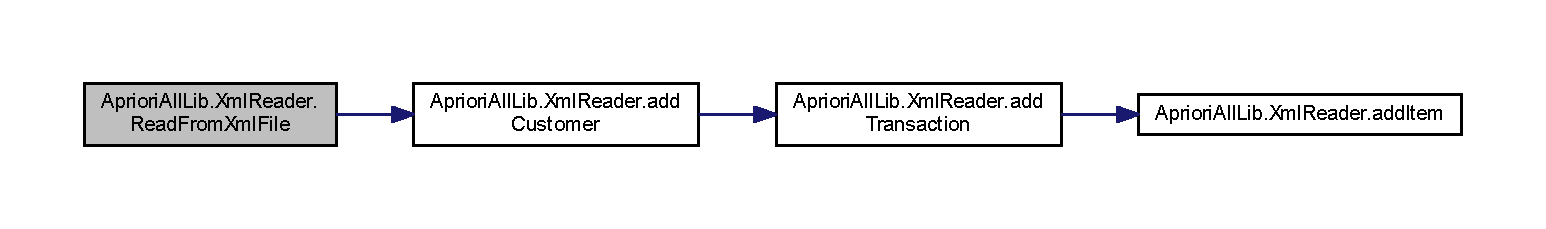
\includegraphics[width=350pt]{class_apriori_all_lib_1_1_xml_reader_ab7285c4d5cee31f7a1001f00f4eeff25_cgraph}
\end{center}
\end{figure}




The documentation for this class was generated from the following file\-:\begin{DoxyCompactItemize}
\item 
D\-:/\-Projects/\-Csharp/\-Mi\-N\-I\-\_\-\-Apriori\-All/\-Apriori\-All\-Lib/\hyperlink{_xml_reader_8cs}{Xml\-Reader.\-cs}\end{DoxyCompactItemize}

\addcontentsline{toc}{part}{Index}
\printindex
\end{document}
